% Adjusting chapter title format for regular (numbered) chapters
\titleformat{\chapter}[display]
  {\normalfont\huge\bfseries\centering}{\chaptertitlename\ \thechapter}{20pt}{\Huge}

% Using similar styling for unnumbered chapters but without "Chapter" prefix
\titleformat{name=\chapter,numberless}
  {\normalfont\huge\bfseries\centering}{}{0pt}{\Huge}

\titlespacing*{\chapter}{0pt}{50pt}{40pt} % Adjust vertical spacing before and after the title


\chapter{Proposed Framework} % Ensures chapter numbering starts correctly

\section*{Proposed Approach}
\begin{figure*}[h]
	\centering
	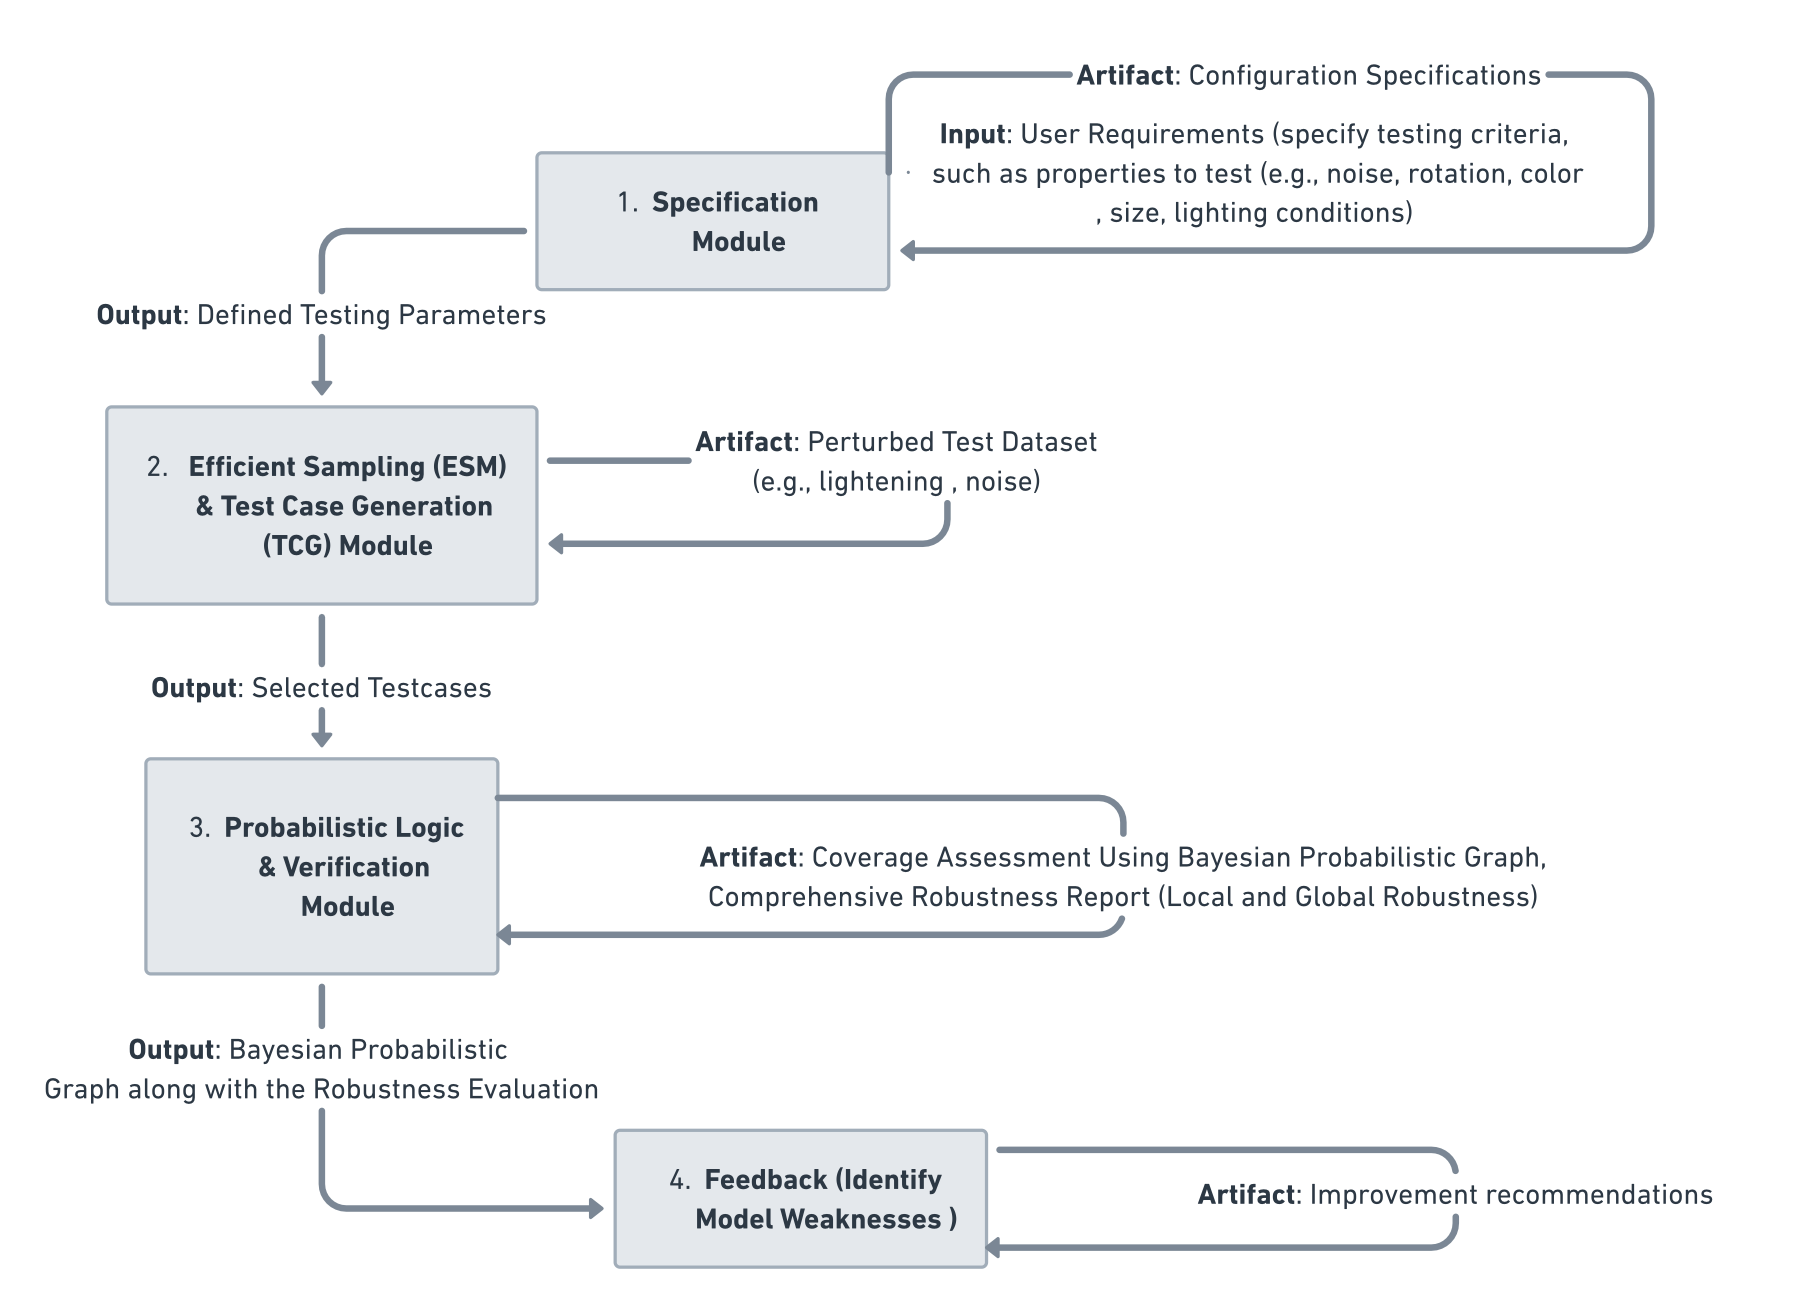
\includegraphics[width=1\textwidth]{overview.png}
	\caption{The outline of proposed approach explains overall flow of work.}
	\label{overview}
\end{figure*}

\subsection{Bayesian Network-based Coverage Metrics}\hypertarget{Bayesian}{}
Two testing coverage metrics are defined in Figure.\ref{Coverage} : the local coverage (LC) and the global coverage (GC). 
\begin{figure*}[h]
	\centering
	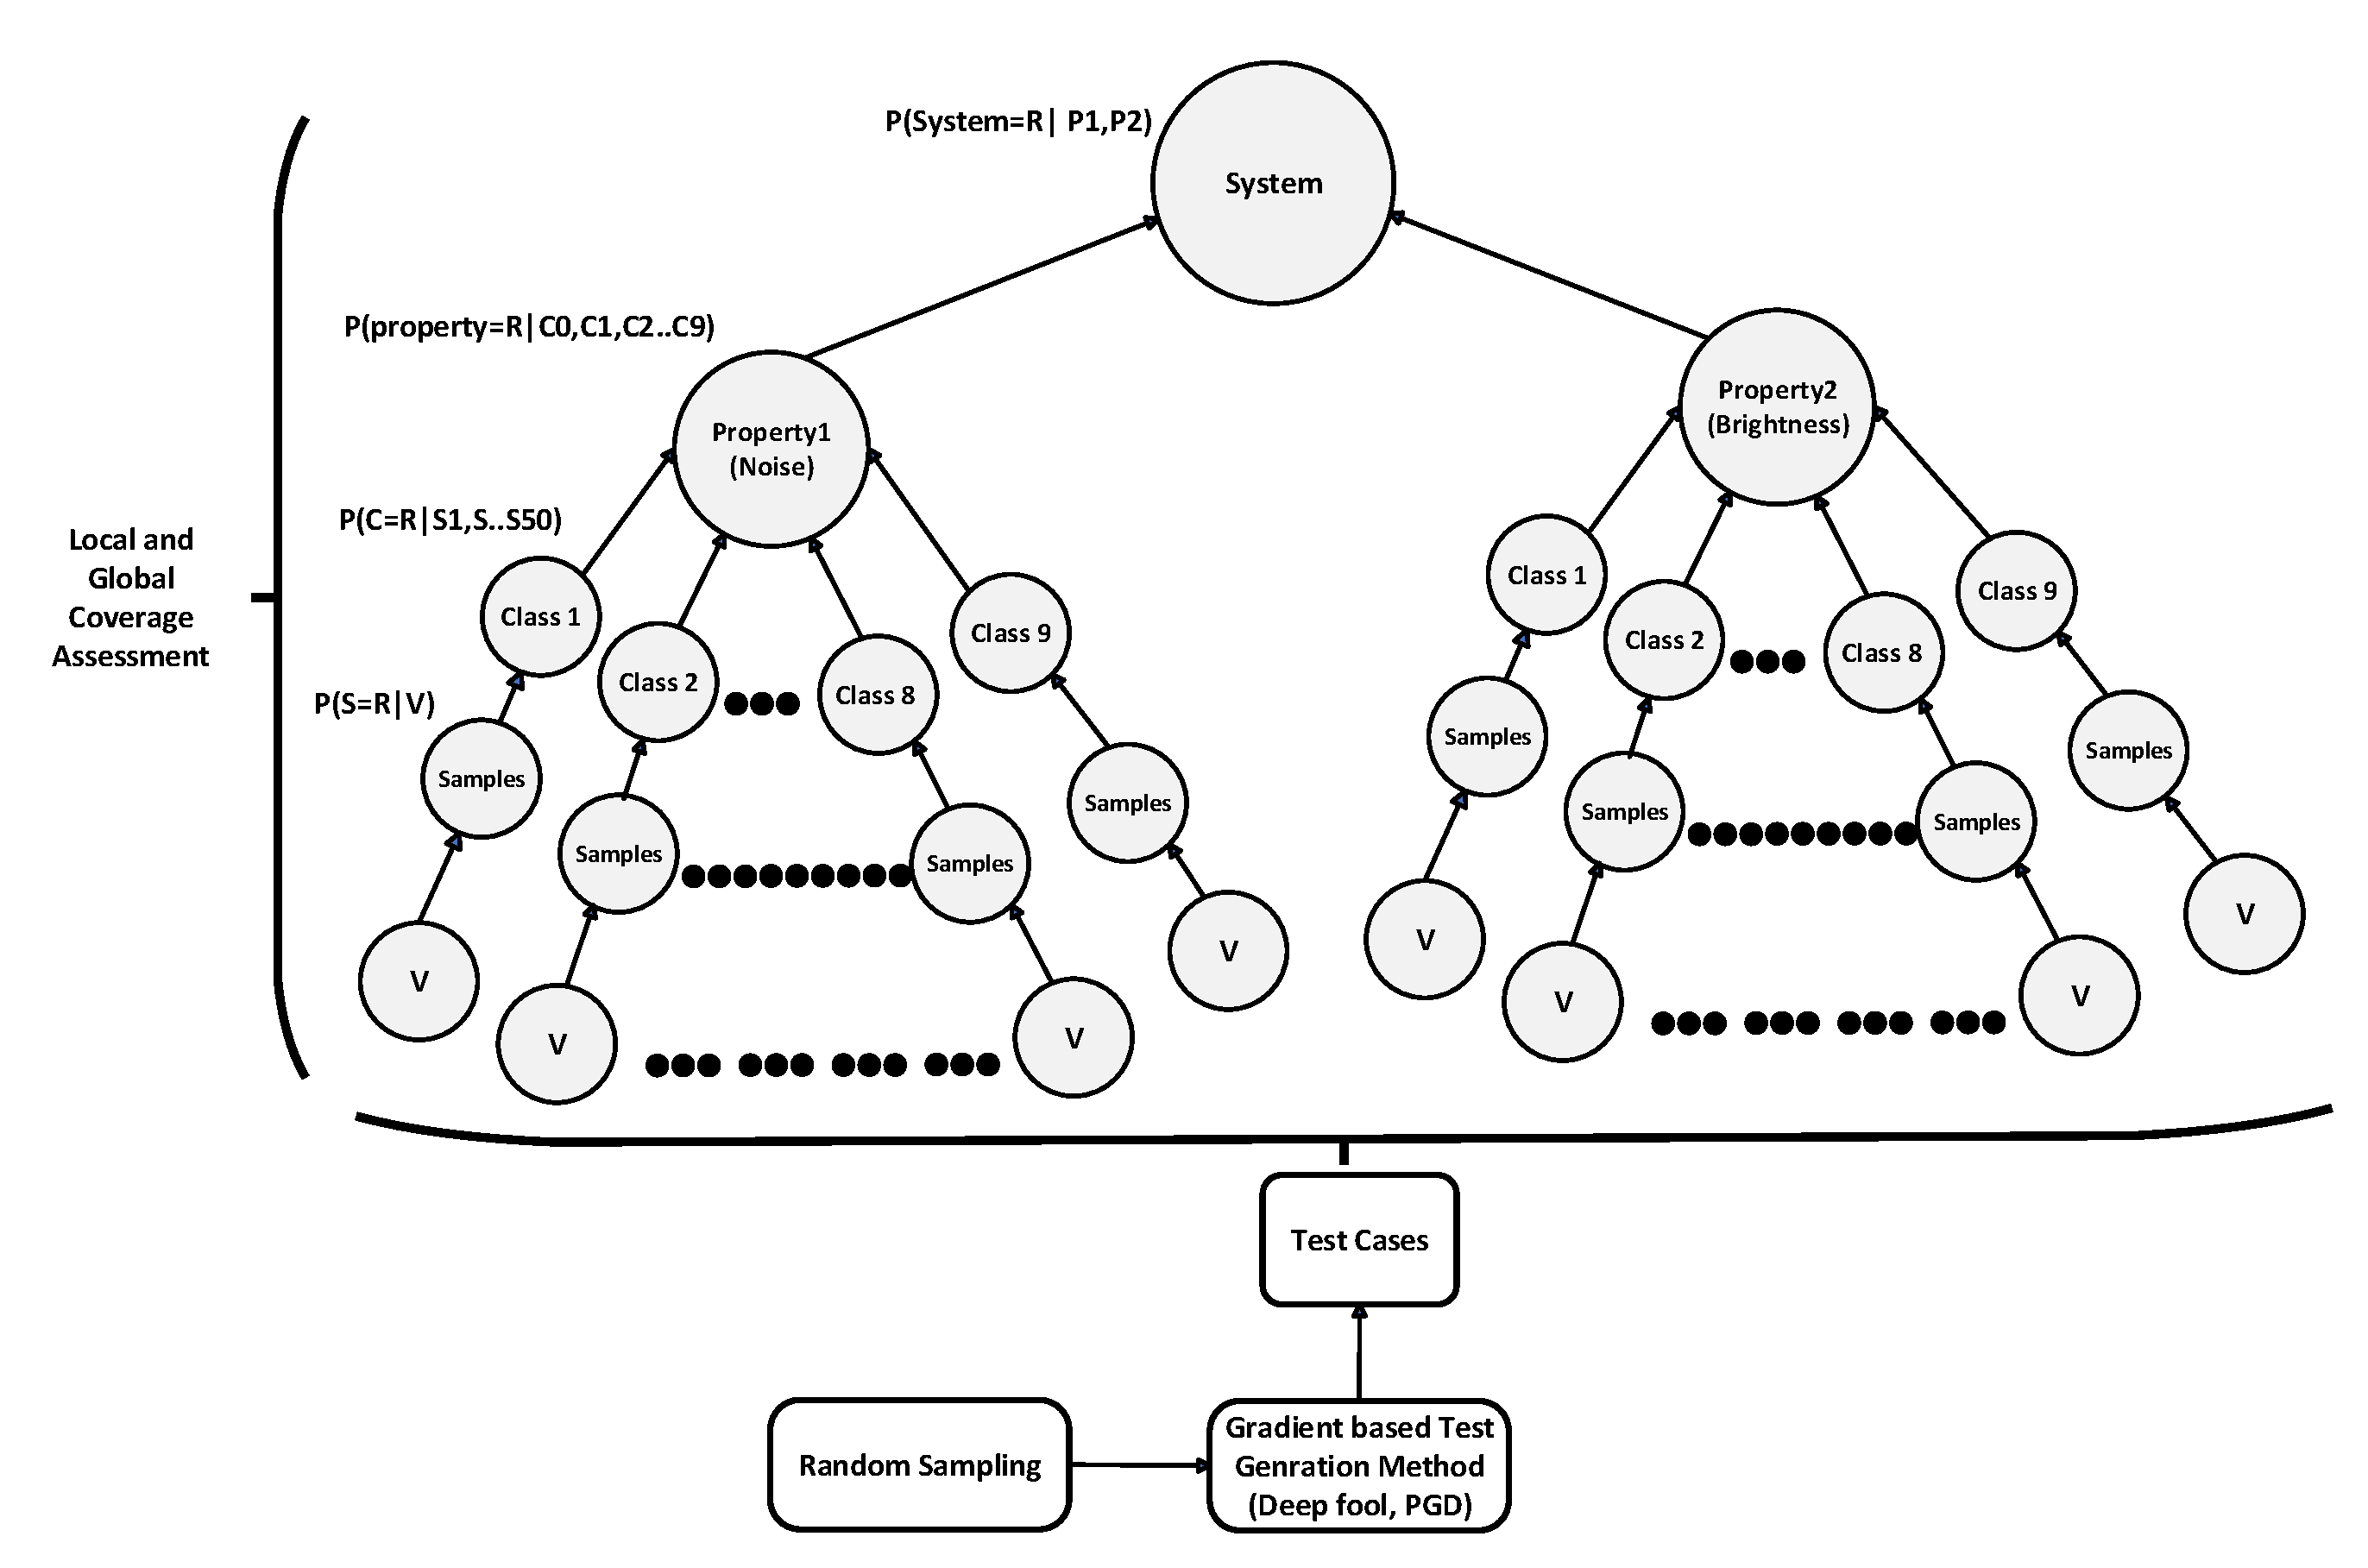
\includegraphics[width=1\textwidth]{ca.pdf}
	\caption{Coverage Assesment (Local and Global)}
	\label{Coverage}
\end{figure*}

\subsection{Gradient based Test Generation}\hypertarget{Gradient}{}

\begin{algorithm}
    \caption{Test Case Generation via Gradient-Based Attacks}
    \begin{tabular}{l l}
    \textbf{Input:} & Model $\mathcal{M}$ with bounds [0, 1], \\
    & Set of images $\mathcal{I} = \{i_1, i_2, \ldots, i_n\}$, \\
    & Corresponding labels $\mathcal{L} = \{l_1, l_2, \ldots, l_n\}$, \\
    & Perturbation magnitudes $\mathcal{E} = \{\epsilon_1, \epsilon_2, \ldots, \epsilon_k\}$, \\
    & Set of attacks $\mathcal{A} = \{A_1, A_2, \ldots, A_m\}$. \\
    \textbf{Output:} & Set of test cases $\bigcup TestCases_{ij}$. \\
    \textbf{Procedure:} & GenerateTestCases($\mathcal{M}$, $\mathcal{I}$, $\mathcal{L}$, $\mathcal{E}$, $\mathcal{A}$) \\
    & \quad \textbf{for} each attack $A_j$ in $\mathcal{A}$ \\
    & \quad \quad \textbf{for} each $\epsilon_i$ in $\mathcal{E}$ \\
    & \quad \quad \quad Generate testcases  $Adv_{ij} = A_j(\mathcal{M}, \mathcal{I}, \epsilon_i)$ \\
    & \quad \quad \quad Verify the $Adv_{ij}$ to obtain $V_{ij}$ \\
    & \quad \quad \quad Evaluate $V_{ij}$ against $\mathcal{L}$ to determine $isRobust_{ij}$ \\
    & \quad \quad \quad Compile test cases $TestCases_{ij} = \{Adv_{ij}, isRobust_{ij}\}$ \\
    & \quad \quad \textbf{end for} \\
    & \quad \textbf{end for} \\
    & \quad \textbf{return} $\bigcup TestCases_{ij}$ \\
    \end{tabular}
    \end{algorithm}
    
